\PassOptionsToPackage{unicode,pdfusetitle}{hyperref}
\PassOptionsToPackage{hyphens}{url}
\PassOptionsToPackage{dvipsnames,svgnames,x11names}{xcolor}

\documentclass[10pt,ignorenonframetext]{beamer}

\usepackage{lmodern}
\usepackage{amssymb,amsmath,mathtools,amsthm}
\usepackage[T1]{fontenc}
\usepackage[utf8]{inputenc}
\usepackage{textcomp} % provide euro and other symbols

\usepackage{pgfpages}

\usepackage{multirow}
\usepackage{csvsimple}
\usepackage{siunitx}

\usepackage{pifont}

% prevent slide breaks in the middle of a paragraph
\widowpenalties 1 10000
\raggedbottom

% Use upquote if available, for straight quotes in verbatim environments
\usepackage{upquote}
\usepackage[]{microtype}
\UseMicrotypeSet[protrusion]{basicmath} % disable protrusion for tt fonts

\usepackage{xcolor}
\usepackage{xurl} % add URL line breaks if available
\usepackage{bookmark}
\usepackage{hyperref}
\hypersetup{%
  colorlinks = true,
  linkcolor  = Cyan4,
  filecolor  = Cyan4,
  citecolor  = SlateBlue4,
  urlcolor   = SlateBlue4
}

% tikz and pgfplots stuff
\usepackage{tikz}
\usetikzlibrary{arrows,shapes,positioning,intersections}
\usepackage{pgfplots}
\usepgfplotslibrary{external,colormaps}
\pgfplotsset{width=7cm,compat=1.11}
%\tikzexternalize

%\usepackage{subfig}
\usepackage{subcaption}
\usepackage{algorithm,algpseudocode}
\usepackage{booktabs}

% bibliography
\usepackage[citestyle=authoryear]{biblatex}
\addbibresource{aistats-slopecd.bib}

\newif\ifbibliography
\setlength{\emergencystretch}{3em} % prevent overfull lines
\setcounter{secnumdepth}{-\maxdimen} % remove section numbering


% redefine part, section, and subsection headers

\raggedbottom
\setbeamertemplate{part page}{
  \centering
  \begin{beamercolorbox}[sep=16pt,center]{part title}
    \usebeamerfont{part title}\insertpart\par
  \end{beamercolorbox}
}
\setbeamertemplate{section page}{
  \centering
  \begin{beamercolorbox}[sep=12pt,center]{part title}
    \usebeamerfont{section title}\insertsection\par
  \end{beamercolorbox}
}
\setbeamertemplate{subsection page}{
  \centering
  \begin{beamercolorbox}[sep=8pt,center]{part title}
    \usebeamerfont{subsection title}\insertsubsection\par
  \end{beamercolorbox}
}

\AtBeginPart{\frame{\partpage}}
\AtBeginSection{\ifbibliography\else\frame{\sectionpage}\fi}
\AtBeginSubsection{\frame{\subsectionpage}}

% beamer configuration
\usecolortheme{dove}
\usefonttheme{professionalfonts}
\usefonttheme{structurebold}
\setbeamertemplate{footline}[frame number]
\setbeamertemplate{caption}[numbered]
\setbeamertemplate{caption label separator}{: }
\setbeamercolor{caption name}{fg=normal text.fg}
\setbeamertemplate{frametitle}{%
  \begin{centering}\insertframetitle\par\end{centering}%
}
\setbeamertemplate{itemize item}{\(\bullet\)}
%\setbeamertemplate{itemize item}[circle]
\setbeamertemplate{itemize subitem}{\(\circ\)}
\setbeamertemplate{itemize subsubitem}{\textendash}
\setbeamerfont{frametitle}{size=\large}
\setbeamertemplate{headline}{\vskip5ex}
\beamertemplatenavigationsymbolsempty
%\setlength{\parskip}{1em} % add paragraph spacing



% operators
\DeclareMathOperator*{\argmax}{arg\,max}
\DeclareMathOperator*{\argmin}{arg\,min}
\DeclareMathOperator{\E}{\text{E}}
\DeclareMathOperator{\var}{var}
\DeclareMathOperator{\cov}{cov}
\DeclareMathOperator{\sign}{sign}
\DeclareMathOperator{\card}{card}
\DeclareMathOperator{\cumsum}{cumsum}
\DeclareMathOperator*{\prox}{prox}

% macros
\newcommand{\pkg}[1]{\textsf{#1}}
\renewcommand{\vec}{\vectorsym}
\newcommand{\mat}{\matrixsym}
\newcommand{\du}{\mathrm{d}}

\makeatletter
\newcommand\notsotiny{\@setfontsize\notsotiny\@vipt\@viipt}
\makeatother



% title block
\title{Lessons Learned from Running a Distance-Based Course in Data
  Visualization}
\subtitle{Cramér Society Fall Meeting 2021}
\author{Johan Larsson}
\institute{Department of Statistics, Lund University}
\date{\today}
\titlegraphic{
\includegraphics{figures/logo.pdf}}

\begin{document}
\frame[noframenumbering,plain]{\titlepage}

\begin{frame}{Overview}
  \tableofcontents
\end{frame}

\section{Course Design}

\begin{frame}{Motivation}
  \begin{itemize}
    \item Data visualization is an integral part of statistics
          \begin{itemize}
            \item Exploring data
            \item Understanding theory
            \item Diagnosing models
            \item Presenting results
          \end{itemize}
    \item Useful in many other professions
  \end{itemize}
\end{frame}

\begin{frame}{Aims}
  \begin{block}{Overall Aim}
    Teach data visualization using modern tools, focusing on both theory and
    practice but with emphasis on the former.
  \end{block}

  \begin{block}{Design-Specific Specific Aims}
    \begin{itemize}
      \item Focus teacher resources on feedback and guidance
      \item Allow asynchronous progress
      \item Enable the course to scale well to many students
      \item Use free (but modern) tools and literature
      \item Encourage student interaction
    \end{itemize}
  \end{block}
\end{frame}

\begin{frame}[c]{Format}
  \begin{columns}[T,onlytextwidth]
    \begin{column}{0.7\linewidth}
      \begin{itemize}
        \item 4 ECTS credits (\(\approx\) 10 hours/week)
        \item Entirely distance-based
        \item Based on R and the R-package ggplot2
        \item Platform: Canvas
        \item Slack workspace for discussions
        \item Zoom for workshops
        \item Freely available literature and tools
      \end{itemize}
    \end{column}
    \begin{column}{0.3\linewidth}
      \centering
      
\includegraphics[width=1.5cm]{figures/r-logo.png}\\
      \vspace{3ex}
      
\includegraphics[width=1.5cm]{figures/ggplot2.png}
      \vspace{3ex}
      
\includegraphics[width=1.5cm]{figures/tidyverse-logo.png}
    \end{column}
  \end{columns}
\end{frame}

\section{Course Content}

\begin{frame}{Course Components}
  \begin{columns}[c,onlytextwidth]
    \begin{column}{0.6\textwidth}
      \begin{block}{Course Activities}
        \begin{itemize}
          \item Pre-Recorded Lectures
          \item Reading Assignments
          \item Worked Examples
          \item Online Workshops
        \end{itemize}
      \end{block}
      \begin{block}{Examination}
        \begin{itemize}
          \item Quizzes
          \item Assignments
          \item Project
        \end{itemize}
      \end{block}
    \end{column}
    \begin{column}{0.4\textwidth}
      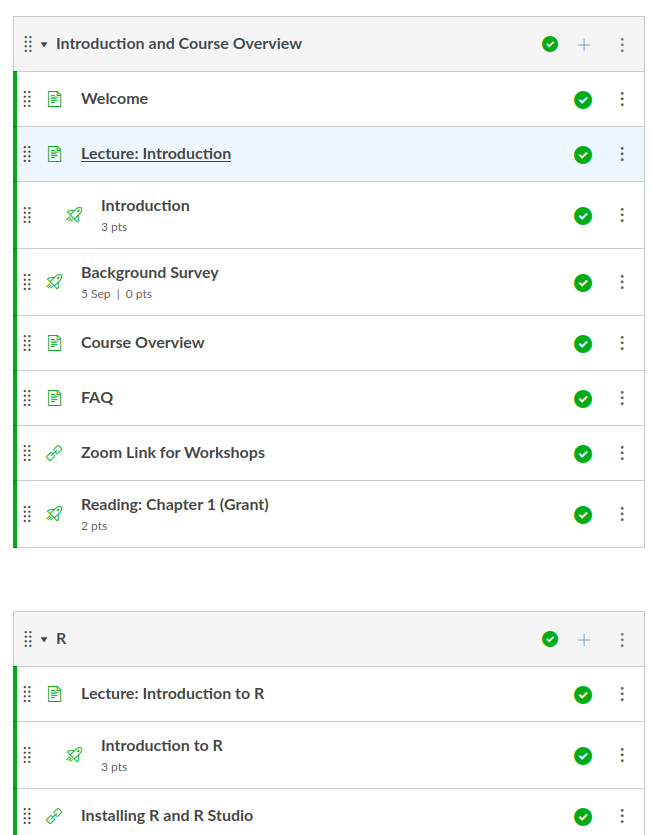
\includegraphics[width=\linewidth]{figures/components.png}
    \end{column}
  \end{columns}
\end{frame}

\begin{frame}{Lectures}
  \begin{columns}[c,onlytextwidth]
    \begin{column}{0.5\linewidth}
      \begin{itemize}
        \item Pre-recorded
        \item Short (5--10 minutes)
        \item Scripted
        \item High production values
      \end{itemize}
    \end{column}
    \begin{column}{0.5\linewidth}
      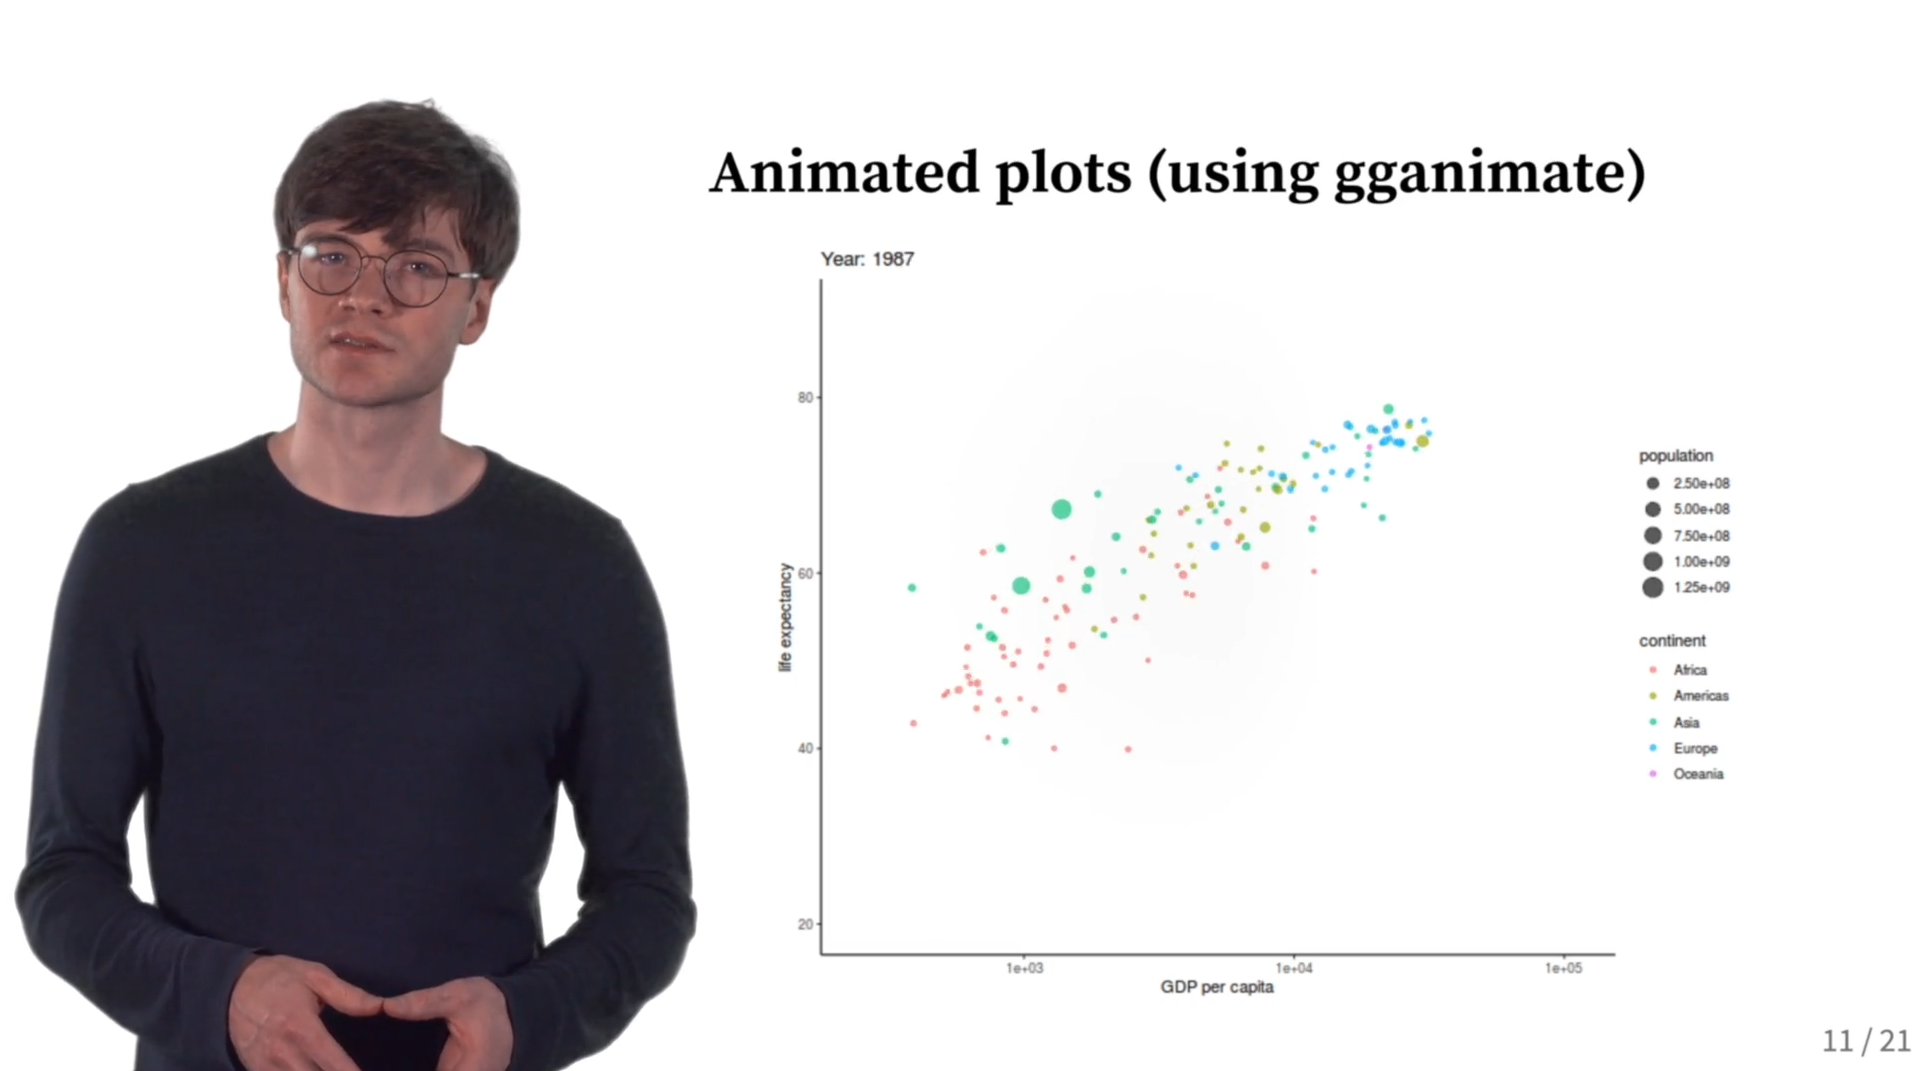
\includegraphics[width=\textwidth]{figures/lecture.png}
    \end{column}
  \end{columns}
\end{frame}

\begin{frame}{Quizzes}
  \begin{columns}[c,onlytextwidth]
    \begin{column}{0.5\linewidth}
      \begin{itemize}
        \item Three types
              \begin{itemize}
                \item Lecture quizzes
                \item Reading quizzes
                \item Practice quizzes
              \end{itemize}
        \item Mostly automatically graded
      \end{itemize}
    \end{column}
    \begin{column}{0.5\linewidth}
      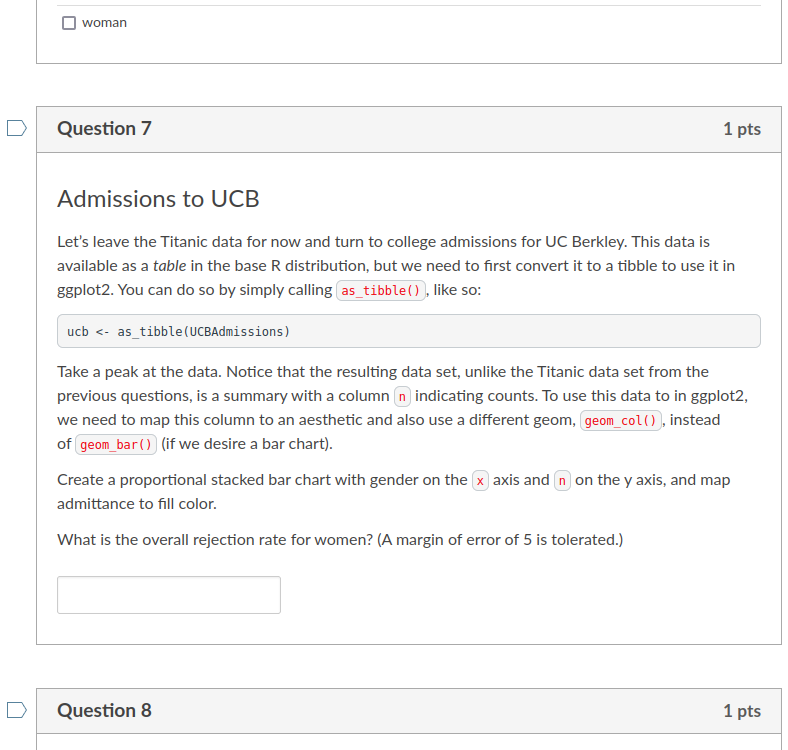
\includegraphics[width=\textwidth]{figures/quiz.png}
    \end{column}
  \end{columns}
\end{frame}

\begin{frame}{Assignments}
  \begin{columns}[c,onlytextwidth]
    \begin{column}{0.5\linewidth}
      \begin{itemize}
        \item Three tasks in each
        \item Progressively freer (and more challenging)
        \item Peer feedback
        \item Short feedback loops
        \item Encourage reproducible submissions (R Markdown)
      \end{itemize}
    \end{column}
    \begin{column}{0.5\linewidth}
      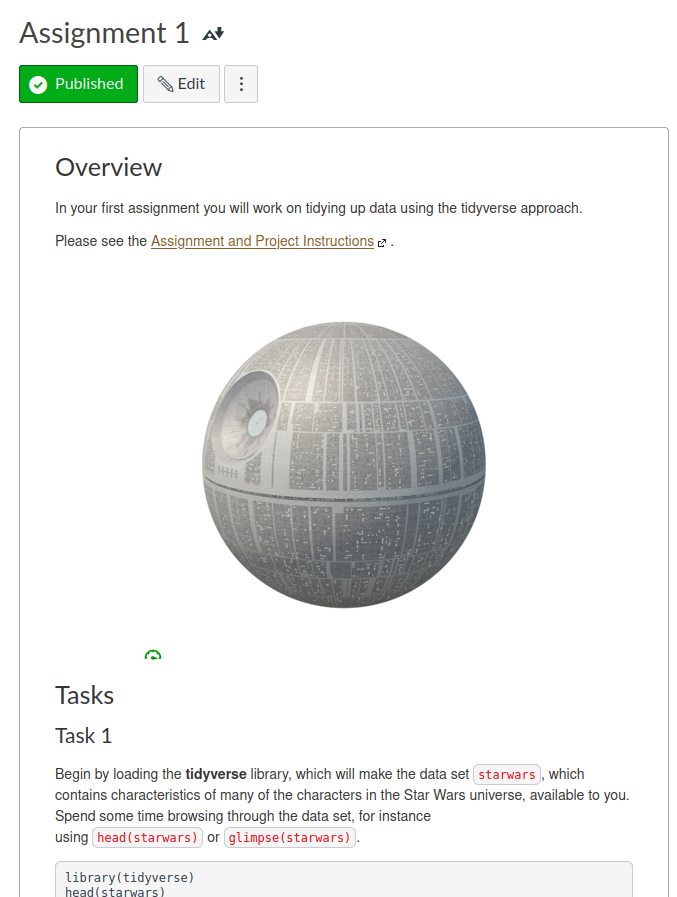
\includegraphics[width=\linewidth]{figures/assignment.png}
    \end{column}
  \end{columns}
\end{frame}

\begin{frame}{Project}
  \begin{columns}[c,onlytextwidth]
    \begin{column}{0.8\linewidth}
      \begin{itemize}
        \item Free choice of "research question"
        \item Free choice of data set (under certain restrictions)
        \item Large variation in results
      \end{itemize}
    \end{column}
    \begin{column}{0.2\linewidth}
    \end{column}
  \end{columns}
\end{frame}

\section{Lessons Learned}

\begin{frame}{Pre-Recorded Lectures: Costly but Worthwhile}
  \begin{itemize}
    \item Excellent student response
    \item Frees up time for real interaction
    \item Large time investment up-front
    \item Best for old (stable) courses
  \end{itemize}
\end{frame}

\begin{frame}{Peer Feedback: Great Value}
  \begin{columns}[c,onlytextwidth]
    \begin{column}{0.6\linewidth}
      \begin{itemize}
        \item Saves time
        \item Fast feedback
        \item From student perspective works best when assignments are free.
              Opposite situation from teacher perspective.
        \item Mixed engagement
      \end{itemize}
    \end{column}
    \begin{column}{0.4\linewidth}
      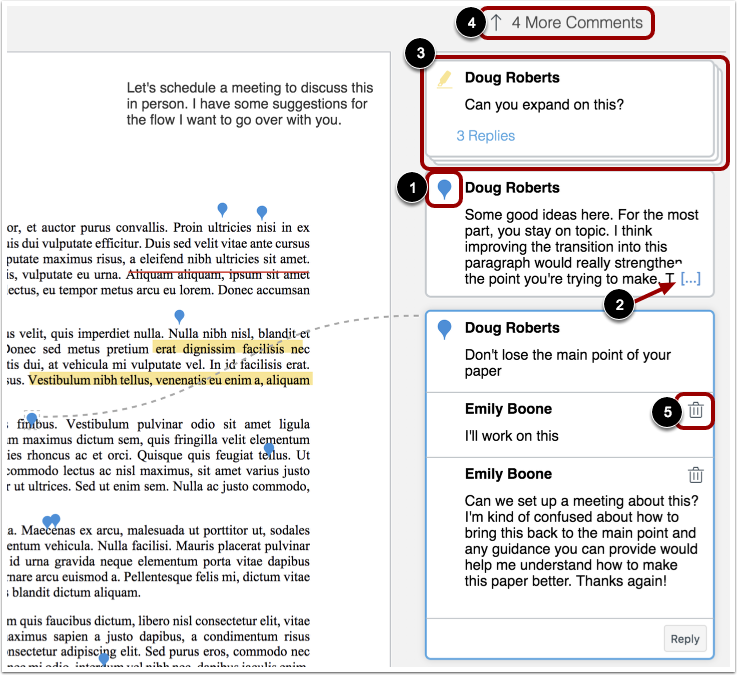
\includegraphics[width=\linewidth]{figures/peer-reviews.png}
    \end{column}
  \end{columns}
\end{frame}

\begin{frame}{Quizzes: Hard to Design, but Useful}
  \begin{itemize}
    \item Hard to design automatically graded quizzes (at least for data
          visualization)
    \item Easy to lose track of students.
          \begin{itemize}
            \item Solution: use a few manually graded tasks
          \end{itemize}
    \item One second attempt seems appropriate, but leads to inflation
    \item "Encourages" students to actually read course literature
  \end{itemize}
\end{frame}

\begin{frame}{Using R: Feasible but not Frictionless}
  \begin{itemize}
    \item Anyone can learn how to use R
    \item Makes assisting students easier
    \item Speeds up revisions
    \item Needs introduction
    \item Divides students into two groups
  \end{itemize}
\end{frame}

\begin{frame}{Retention}
  \begin{itemize}
    \item Register many students! \(\approx\) 50\% drop out.
    \item
  \end{itemize}
\end{frame}

\begin{frame}{Asynchronicity: A Mixed Bag}
  \begin{itemize}
    \item Great for some students
    \item Does not combine so well with peer (and general) feedback
  \end{itemize}
  \vspace{15ex}
  \begin{center}
    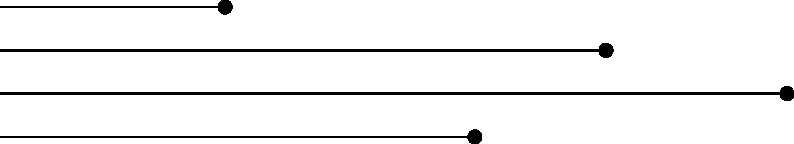
\includegraphics[width=0.7\linewidth]{figures/async.pdf}
  \end{center}
\end{frame}

\begin{frame}{Conclusions}
  \begin{itemize}
    \item Works well overall
    \item Peer reviews are great
    \item Quizzes are efficient in stimulating learning
    \item Automatic grading is useful but hard to design well
  \end{itemize}
\end{frame}

% \begin{frame}[allowframebreaks]{References}
%   \bibliographytrue
%   \printbibliography[heading=none]
% \end{frame}

\end{document}
